% Source release commit: 77a4eb55bce97f7ac736ac36099e70a6d5135506
% Release manifest SHA-256: 2e0e1a28b6916d84b450eaf9218e344f1e10d9d91533ae43deed3677756820c4
% Generated by dose_main_release; descriptive reporting, not new inference.
\newcommand{\DoseMainCalibrationTrials}{204}
\newcommand{\DoseMainComplete}{1}
\newcommand{\DoseMainControlOneNegativeN}{32}
\newcommand{\DoseMainControlOneNegativeQualityFlagged}{1}
\newcommand{\DoseMainControlOnePositiveN}{32}
\newcommand{\DoseMainControlOnePositiveQualityFlagged}{3}
\newcommand{\DoseMainControlTwoNegativeN}{32}
\newcommand{\DoseMainControlTwoNegativeQualityFlagged}{3}
\newcommand{\DoseMainControlTwoPositiveN}{32}
\newcommand{\DoseMainControlTwoPositiveQualityFlagged}{4}
\newcommand{\DoseMainControlThreeNegativeN}{32}
\newcommand{\DoseMainControlThreeNegativeQualityFlagged}{1}
\newcommand{\DoseMainControlThreePositiveN}{32}
\newcommand{\DoseMainControlThreePositiveQualityFlagged}{3}
\newcommand{\DoseMainPaperControlOneEstimate}{-0.094}
\newcommand{\DoseMainPaperControlOneHigh}{0.212}
\newcommand{\DoseMainPaperControlOneLow}{-0.374}
\newcommand{\DoseMainPaperControlOneNegativeMissing}{0}
\newcommand{\DoseMainPaperControlOneNegativeYes}{26}
\newcommand{\DoseMainPaperControlOnePositiveMissing}{0}
\newcommand{\DoseMainPaperControlOnePositiveYes}{29}
\newcommand{\DoseMainPaperControlTwoEstimate}{-0.094}
\newcommand{\DoseMainPaperControlTwoHigh}{0.187}
\newcommand{\DoseMainPaperControlTwoLow}{-0.347}
\newcommand{\DoseMainPaperControlTwoNegativeMissing}{0}
\newcommand{\DoseMainPaperControlTwoNegativeYes}{26}
\newcommand{\DoseMainPaperControlTwoPositiveMissing}{0}
\newcommand{\DoseMainPaperControlTwoPositiveYes}{29}
\newcommand{\DoseMainPaperControlThreeEstimate}{-0.125}
\newcommand{\DoseMainPaperControlThreeHigh}{0.193}
\newcommand{\DoseMainPaperControlThreeLow}{-0.410}
\newcommand{\DoseMainPaperControlThreeNegativeMissing}{0}
\newcommand{\DoseMainPaperControlThreeNegativeYes}{23}
\newcommand{\DoseMainPaperControlThreePositiveMissing}{0}
\newcommand{\DoseMainPaperControlThreePositiveYes}{27}
\newcommand{\DoseMainPaperQualityPass}{1}
\newcommand{\DoseMainPaperSpecificityEstimate}{0.052}
\newcommand{\DoseMainPaperSpecificityHigh}{0.559}
\newcommand{\DoseMainPaperSpecificityLow}{-0.486}
\newcommand{\DoseMainPaperTargetEstimate}{-0.052}
\newcommand{\DoseMainPaperTargetHigh}{0.101}
\newcommand{\DoseMainPaperTargetLow}{-0.201}
\newcommand{\DoseMainPaperTargetNegativeMissing}{0}
\newcommand{\DoseMainPaperTargetNegativeYes}{82}
\newcommand{\DoseMainPaperTargetPositiveMissing}{0}
\newcommand{\DoseMainPaperTargetPositiveYes}{87}
\newcommand{\DoseMainPaperZeroMissing}{0}
\newcommand{\DoseMainPaperZeroYes}{81}
\newcommand{\DoseMainSecondControlOneEstimate}{-0.188}
\newcommand{\DoseMainSecondControlOneHigh}{0.169}
\newcommand{\DoseMainSecondControlOneLow}{-0.496}
\newcommand{\DoseMainSecondControlOneNegativeMissing}{0}
\newcommand{\DoseMainSecondControlOneNegativeYes}{9}
\newcommand{\DoseMainSecondControlOnePositiveMissing}{0}
\newcommand{\DoseMainSecondControlOnePositiveYes}{15}
\newcommand{\DoseMainSecondControlTwoEstimate}{-0.125}
\newcommand{\DoseMainSecondControlTwoHigh}{0.244}
\newcommand{\DoseMainSecondControlTwoLow}{-0.463}
\newcommand{\DoseMainSecondControlTwoNegativeMissing}{0}
\newcommand{\DoseMainSecondControlTwoNegativeYes}{15}
\newcommand{\DoseMainSecondControlTwoPositiveMissing}{0}
\newcommand{\DoseMainSecondControlTwoPositiveYes}{19}
\newcommand{\DoseMainSecondControlThreeEstimate}{-0.031}
\newcommand{\DoseMainSecondControlThreeHigh}{0.309}
\newcommand{\DoseMainSecondControlThreeLow}{-0.363}
\newcommand{\DoseMainSecondControlThreeNegativeMissing}{0}
\newcommand{\DoseMainSecondControlThreeNegativeYes}{12}
\newcommand{\DoseMainSecondControlThreePositiveMissing}{0}
\newcommand{\DoseMainSecondControlThreePositiveYes}{13}
\newcommand{\DoseMainSecondQualityPass}{1}
\newcommand{\DoseMainSecondSpecificityEstimate}{0.219}
\newcommand{\DoseMainSecondSpecificityHigh}{0.834}
\newcommand{\DoseMainSecondSpecificityLow}{-0.448}
\newcommand{\DoseMainSecondTargetEstimate}{0.104}
\newcommand{\DoseMainSecondTargetHigh}{0.298}
\newcommand{\DoseMainSecondTargetLow}{-0.098}
\newcommand{\DoseMainSecondTargetNegativeMissing}{0}
\newcommand{\DoseMainSecondTargetNegativeYes}{49}
\newcommand{\DoseMainSecondTargetPositiveMissing}{0}
\newcommand{\DoseMainSecondTargetPositiveYes}{39}
\newcommand{\DoseMainSecondZeroMissing}{0}
\newcommand{\DoseMainSecondZeroYes}{36}
\newcommand{\DoseMainSelectedDose}{0.25}
\newcommand{\DoseMainTargetNegativeN}{96}
\newcommand{\DoseMainTargetNegativeQualityFlagged}{8}
\newcommand{\DoseMainTargetPositiveN}{96}
\newcommand{\DoseMainTargetPositiveQualityFlagged}{8}
\newcommand{\DoseMainTrials}{480}
\newcommand{\DoseMainZeroN}{96}
\newcommand{\DoseMainZeroQualityFlagged}{7}

% Observed cap counts, not population estimates.
\newcommand{\DoseFollowupFinalCaps}{6}
\newcommand{\DoseFollowupInductionCaps}{47}
\newcommand{\DoseFollowupTokenCap}{512}

\subsection{A quality-selected steering dose}
\label{sec:dose-followup}

The dose follow-up did not establish the predefined large, target-specific
increase in report labels. At the selected dose, the negative-minus-positive
target contrast was \(\DoseMainSecondTargetEstimate{}
[\DoseMainSecondTargetLow{}, \DoseMainSecondTargetHigh{}]\) under the primary
notebook classifier and \(\DoseMainPaperTargetEstimate{}
[\DoseMainPaperTargetLow{}, \DoseMainPaperTargetHigh{}]\) under the secondary paper rubric
(individual conservative 95\% intervals). The primary upper bound,
\(\DoseMainSecondTargetHigh{}\), was only just below the predeclared 0.30
threshold. This is a narrow exclusion at one selected dose, not robust
exclusion across doses. The primary target-minus-mean-control contrast was
\(\DoseMainSecondSpecificityEstimate{}
[\DoseMainSecondSpecificityLow{}, \DoseMainSecondSpecificityHigh{}]\), leaving
target specificity unresolved (Figure~\ref{fig:dose-followup}).

A separate \DoseMainCalibrationTrials{}-trial calibration selected dose
\DoseMainSelectedDose{} from four tested levels using heuristic quality
criteria rather than nonzero-dose report rates. Each higher tested dose failed
at least one target or control quality check and was not carried forward.
The target mixture used features 41533, 58667, and 30686. Each feature's
reference scale was the largest category mean of per-text maxima in the
designed NF4 mapping set, not a natural-corpus peak. Confirmation comprised
\DoseMainTrials{} trials in 96 paired seed blocks: untreated generation,
both edit signs for the target, and both signs for one of three fixed,
norm-matched control panels (32 blocks per panel). The technical continuation
carried calibration and selection forward unchanged.

The quality-rule amendment followed earlier calibration results. It treated
first-turn truncation at \DoseFollowupTokenCap{} tokens as exposure metadata,
while final-turn truncation remained a quality failure. In confirmation,
\DoseFollowupInductionCaps{} induction turns and \DoseFollowupFinalCaps{}
final turns reached that cap. The selected-dose main sample passed the
specified heuristic quality rule; this is not human coherence validation.
These results concern automated labels under this finite-exposure public
operator, not consciousness or removal of a semantic representation.

\begin{figure}[t]
\centering
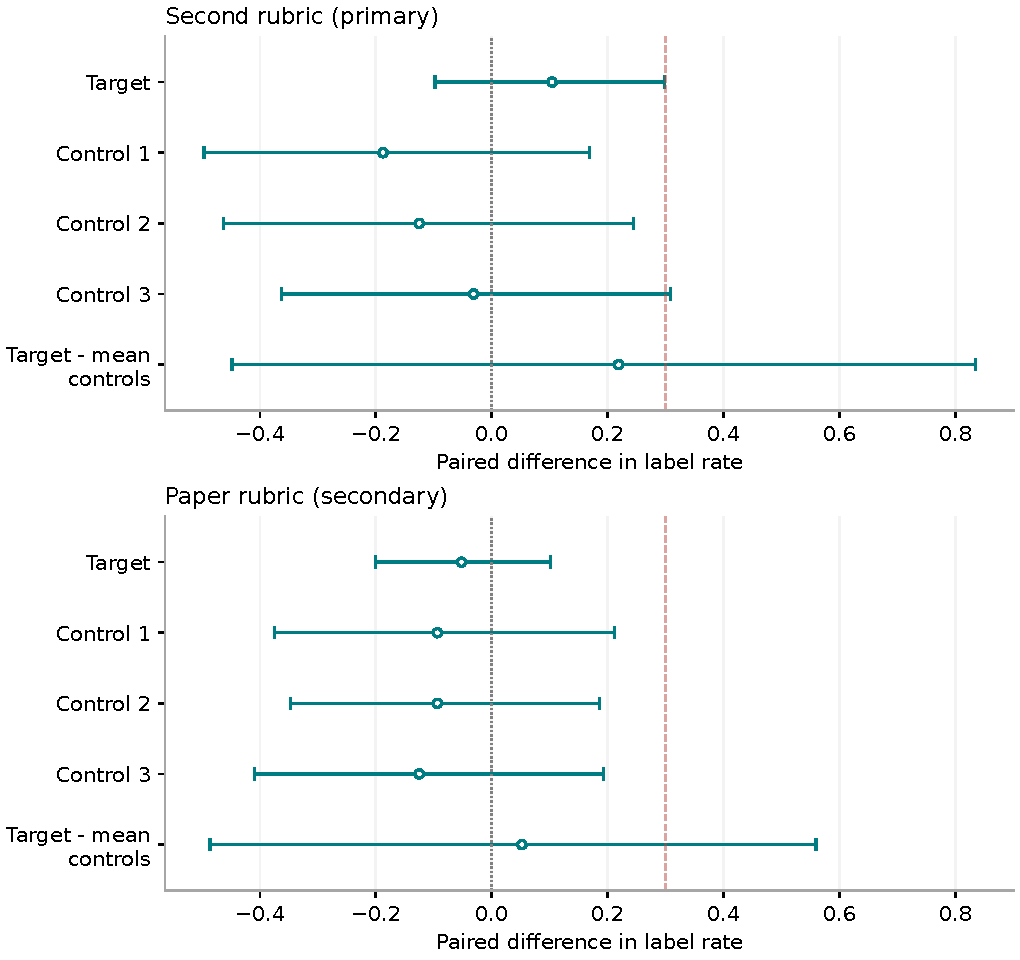
\includegraphics[width=\linewidth]{../evidence/dose_followup/main_contrasts.pdf}
\caption{Paired label contrasts at the quality-selected dose. ``Second rubric''
identifies the notebook classifier used in the earlier analyses. Open circles
show negative-minus-positive estimates, with conservative 95\% paired-discordance
Clopper--Pearson bounds. Both rubrics, all three fixed control panels, and the
target-minus-equal-mean-control contrast are shown. Target contrasts use 96
paired blocks; each control panel uses 32. The dashed 0.30 line is the target
threshold, not a specificity threshold. Intervals are individual, not
simultaneous across contrasts or rubrics; the control-panel comparisons are
descriptive. Calibration is separate from these main-trial estimates.}
\label{fig:dose-followup}
\end{figure}
